\chapter{Results}
\label{chap:results}

In the following chapter we will first describe the experimental setup, the assumptions used. Further we will perform brief dataset description. In the main part we will focus on the evaluation of different model variants and their comparison and evaluation of impact of each additional extension on the model performance. Lastly, we will briefly approximate the dependence of our model performance on the number of experiments in our train dataset and number of neurons taken from the original SNN of cat.

Note that in this chapter we will use the abbreviations for the model layers as follows: X\_ON, X\_OFF for LGN ON and OFF cell populations, V1\_Exc\_L4 and V1\_Inh\_L4 for V1 excitatory and inhibitory cell populations in layer 4, V1\_Exc\_L23 and V1\_Inh\_L23 for V1 excitatory and inhibitory cell populations in layer 2/3. These abbreviations will be used throughout the whole chapter and reflects the exact naming of the layers in our model implementation.

\section{Experimental Setup and Technicalities}
\label{sec:experimental_setup}
In all the experimental runs if not stated differently we use the model setup and artificial dataset closely described in the Chapter~\ref{chap:methods}.

Apart from the setup closely described in the previous chapter there are a few of the general truth parameters that we typically empirically selected based on our experience from the initial phases of the model development either because of the technical limitations, such as appropriate GPU machines (or long waiting times), memory constraints etc., or some other difficulties specific to our model and dataset. In selection of these parameters we typically have decided empirically the ideal values as the comprehensive experimental confirmation would be typically too demanding in terms of the computational power and time, and typically we do not expect that these would have significant effect on the results of our study. It is worth to mention though, that these might be fine-tuned in the future research for optimization.

Example of such a parameter is the batch size. As mentioned in Section~\ref{sec:artificial_dataset} our dataset data are split into the samples representing the experiments. These needs to be split into the batches. In our experimental setup we have empirically chosen the batch size to be $50$. This size has been selected from a various reasons. As the RNN training process is being done sequentially on the temporal data it is usually demanding in time necessary for the training step as the properties does not really support parallel backpropagation computation. From this reason there is only a limited possibility to reasonable speed up the computations. One of this is selection of the bigger batch size that enables a parallel backpropagation step across the batch of experiments if executed on the GPUs. On the other hand, with the increasing batch size there also rises demand for the memory usage. The memory consumption is especially problematic while using the RNN neuronal variants closely described in Section~\ref{subsec:additional_modules} that requires truncated backpropagation throughout time (TBPTT) computation that significantly increases memory demands needed for the training of the model that is intensified by the small shared NN modules instead of activation functions. This problem is partially solved by merging the time bins into 20~ms time bins and thus reducing the necessity for applying TBPTT in large number of time steps as mentioned in Section~\ref{subsubsec:time_bins_merging}, however, it does not solve the memory problems fully. Additionally as mentioned in the Section~\ref{subsubsec:subset_selection} we have been forced for the same reasons to select only subset 10\% of the artificial neurons from our template SNN model from each layer in order to meet the memory constraints. Based on these we have then finally selected to choose batch size $50$ to maintain the same conditions in all experiments as possible and that fulfils the memory constraints also for the most memory demanding model variants such as the one using synaptic depression module (Section~\ref{subsubsec:synaptic_depression}).

Additionally to batch size, we also apply gradient clipping to secure the exploding gradient problem. In all our experiments it is applied 10,000. This value has been selected as a sanity boundary to ensure the gradient updates applied during model training do not overflow the floating number representation in our model implementation and do not cause the errors caused by overflowing numbers. It has been empirically tested that this gradient clipping has not been necessary to apply throughout all our variants of the model used in the experiment. It is used mainly because there has been such problems especially at the initial stages of the model training while using activation function different from our current LeakyTanh. This problematic is also briefly mentioned in the Section~\ref{subsubsec:leakytanh}. Overall, the effect of the gradient clipping in our setup should not have a significant impact on the model performance.

At the end, we would like to mention the recommended machines on which we performed our experiments and are tested to perform without problems in our model. Majority of the experiments has been performed on the Metacentrum computational server. While some of the model variants does not require high amount of the GPU RAM we typically selected the devices with at least 40~GB GPU RAM as these GPUs are typically optimized for large tensor operations in DNN related computation, additionally in the models that require TBPTT it is almost necessary to use at least 40~GB GPU RAM. Alongside with this we worked with at least 8 CPU Cores with 100~GB RAM.

\section{Dataset Overview}
\label{sec:dataset_overview}

In this section we will focus on statistical analysis of our dataset and we will investigate the influence of our dataset simplifications on our data. We will focus first on the influence of merging time bins from 1~ms to 20~ms and then we will focus on the influence of selecting random subset of 10\% neurons. Implementation of all tests performed during the dataset overview can be found in the appropriate files in the supplementary materials to the text of the thesis and in the github repository of the project.

\subsection{Time Bin Merging Analysis}
\label{subsec:time_bin_merging_analysis}
As already stated in Section~\ref{subsubsec:time_bins_merging} we merge our time intervals from 1~ms time bins to 20~ms time bins to speed up the calculations and ideally also to remove the noisiness of our data while still capturing reasonable temporal resolution. We will perform our experiments on time bin sizes 1~ms, 5~ms, 10~ms, 15~ms and 20~ms. We should also mention that it was not really suitable to test this on the larger subset of different time bins as the usage of each time bin requires computationally demanding processing of the whole dataset that merges the time bins and then stored the new dataset that also requires significant amount of memory and is not suitable for us to prepare more different subsets. It is done to massively speed up the model training and to reduce the memory consumption. 

\subsubsection{Total Spike Counts Across Time Bins}
\label{subsubsec:spike_counts_time_bins}

First, we will focus on the comparison of the distribution of spike counts across all time bins with the different. We claim the following:

\begin{claim}[Distribition of Spike Counts Across All Time Bins]
    The distribution of spike counts across all time bins remains similar for time bin sizes $\{1, 5, 10, 15, 20\}$. This indicates that the temporal behavior of the neuronal responses stays roughly the same.
\end{claim}
\label{claim:tim_bin_counts}

Our claim is that if the time binning maintains mainly the binary like properties of the data it also mostly maintains the temporal properties of the sequences. First, let us compare the distribution of spike counts across all time bins for different binning sizes that are depicted in the Table~\ref{tab:train_bin_count_distribution} for the train dataset and Table~\ref{tab:test_bin_count_distribution} for the test dataset.

\begin{table}
    \centering\footnotesize\sf
    \begin{tabular}{cccccc}
    \toprule
        Spike Count & 1 ms & 5 ms & 10 ms & 15 ms & 20 ms \\
        \midrule
        0 & 0.9944 & 0.9727 & 0.9491 & 0.9287 & 0.9105 \\
        1 & 0.0056 & 0.0266 & 0.0460 & 0.0598 & 0.0710 \\
        2 & 0.0000 & 0.0007 & 0.0046 & 0.0100 & 0.0147 \\
        3 & 0.0000 & 0.0000 & 0.0003 & 0.0013 & 0.0032 \\
        4 & 0.0000 & 0.0000 & 0.0000 & 0.0001 & 0.0005 \\
        5 & 0.0000 & 0.0000 & 0.0000 & 0.0000 & 0.0001 \\
    \addlinespace % a nice non-intrusive separator of data groups (or final table sums)
    \bottomrule
    \end{tabular}
    \caption{\textbf{Train spike count distribution:} This table depicts the ratios of number of spikes in one time bin for different time bin sizes in train dataset. Spike counts above 5 are omitted as they are present only in minority of examples and does not really affect the distribution.}
    \label{tab:train_bin_count_distribution}
\end{table}
    

\begin{table}
    \centering\footnotesize\sf
    \begin{tabular}{cccccc}
    \toprule
        Spike Count & 1 ms & 5 ms & 10 ms & 15 ms & 20 ms \\
    \midrule
        0 & 0.9944 & 0.9728 & 0.9493 & 0.9290 & 0.9107 \\
        1 & 0.0056 & 0.0265 & 0.0458 & 0.0597 & 0.0710 \\
        2 & 0.0000 & 0.0007 & 0.0045 & 0.0099 & 0.0146 \\
        3 & 0.0000 & 0.0000 & 0.0003 & 0.0013 & 0.0032 \\
        4 & 0.0000 & 0.0000 & 0.0000 & 0.0001 & 0.0005 \\
        5 & 0.0000 & 0.0000 & 0.0000 & 0.0000 & 0.0001 \\
    \addlinespace % a nice non-intrusive separator of data groups (or final table sums)
    \bottomrule
    \end{tabular}
    \caption{\textbf{Test spike count distribution:} This table depicts the ratios of number of spikes in one time bin for different time bin sizes in test dataset. Spike counts above 5 are omitted as they are present only in minority of examples and does not really affect the distribution.}
    \label{tab:test_bin_count_distribution}
\end{table}

As we can see the distributions are very similar between train and test dataset furthermore we can see that there has not been very serious shift in the spike count distribution across time bins as majority remained either 0 or 1 and only a few of them contain more than 1 spike. Namely for the time bin size of our interest 20~ms there is only approximately 1.5\% of time bins that contain at least 2 spikes. However, what changed significantly is the amount of time bins where at least one spike occurred that changed from roughly 0.6\% to roughly 7\% for time bin size 20~ms. This is a clear sign that the sparsity of our dataset significantly dropped and since the distribution does not really change that much it might be also a sign that this time bin size is ideal for balancing the temporal resolution and dataset size since we reduce sparsity of our dataset. For comparison of the time bin count distribution we have also prepared plots of the spike counts for each time bin variant for each neuronal population. These plots can be seen in the Figure~\ref{fig:spike_count_distribution_train} for train dataset and in the Figure~\ref{fig:spike_count_distribution_test} for the test dataset.

\begin{figure}
    \centering
    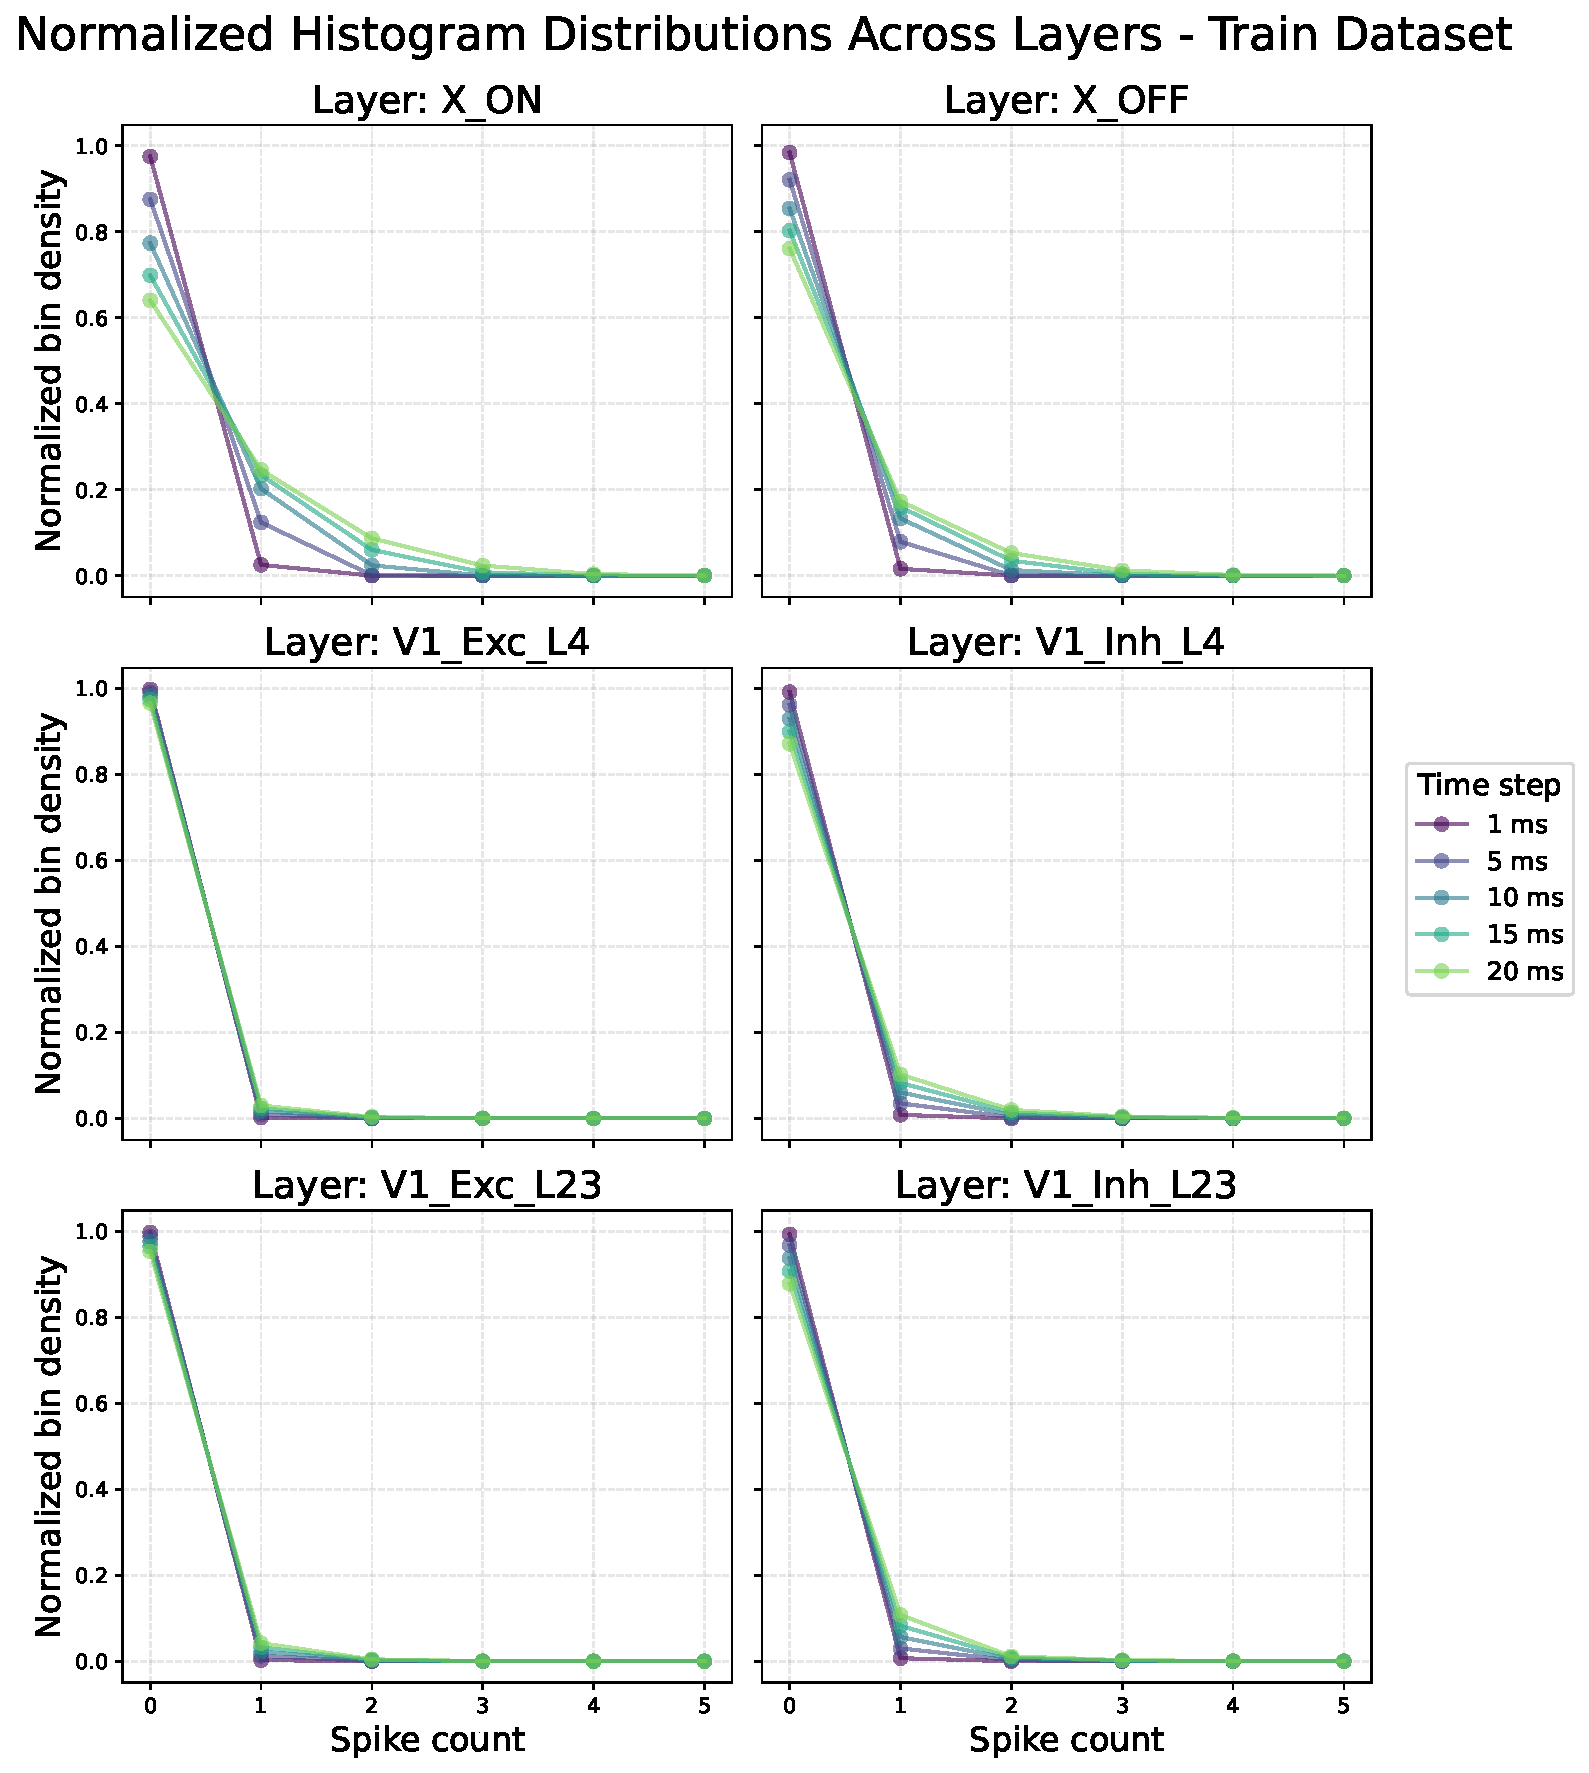
\includegraphics[width=\linewidth]{img/plots/time_step_counts_train.pdf}
    \caption{The evolution of the spike counts in single time bin with rise of the time bin size across all neuronal populations for train dataset.}
    \label{fig:spike_count_distribution_train}
\end{figure}

\begin{figure}
    \centering
    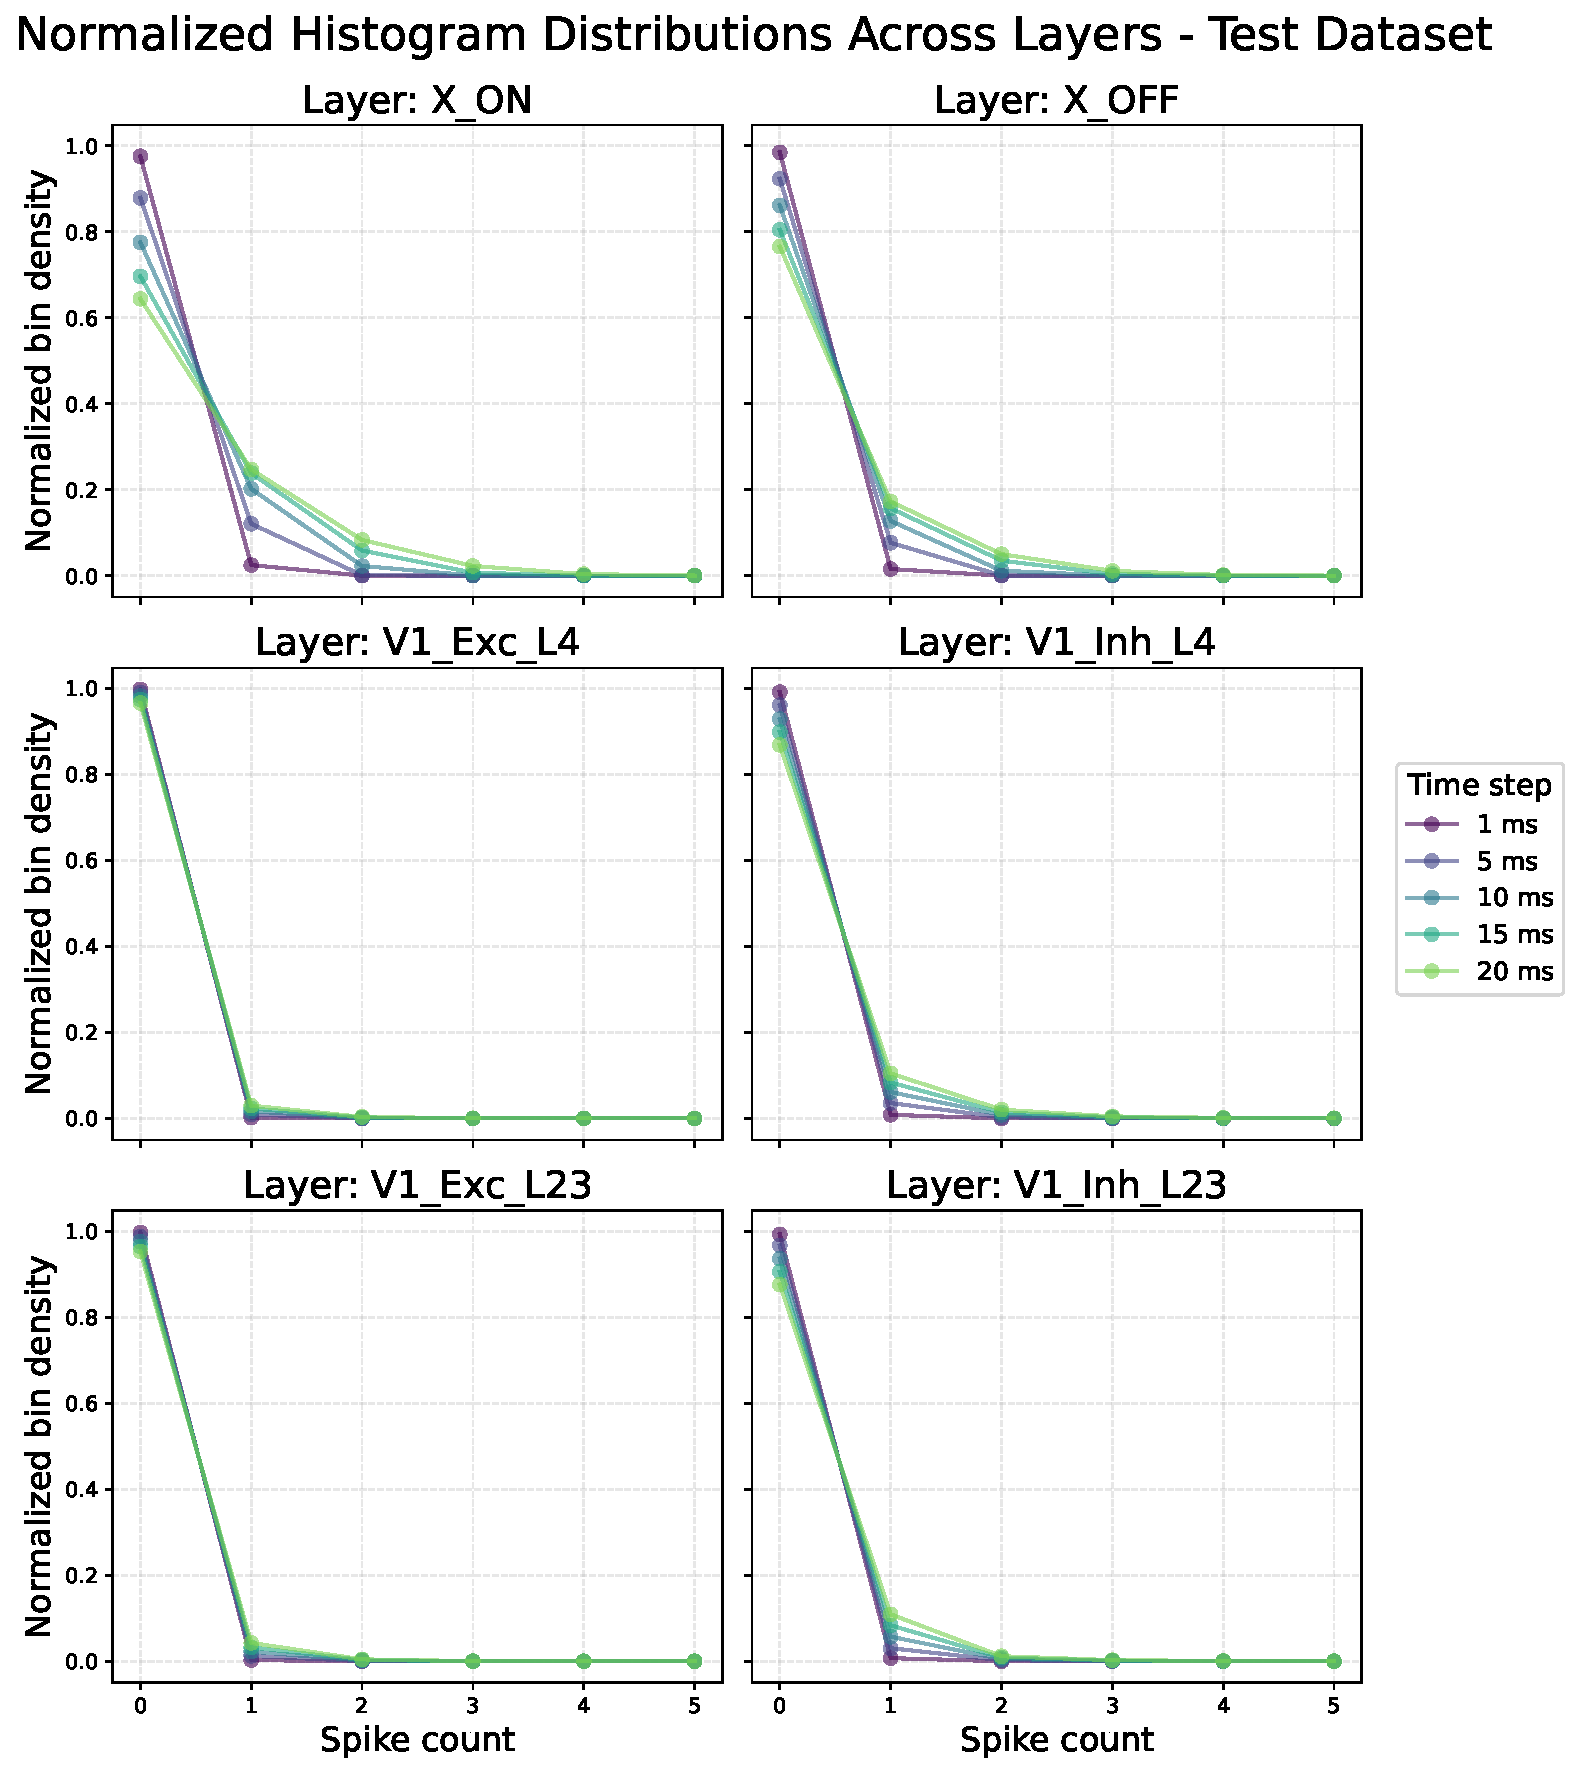
\includegraphics[width=\linewidth]{img/plots/time_step_counts_test.pdf}
    \caption{The evolution of the spike counts in single time bin with rise of the time bin size across all neuronal populations for test dataset.}
    \label{fig:spike_count_distribution_test}
\end{figure}

\subsubsection{Spike Count Distribution Across Time}
\label{subsubsec:spike_time_distribution}
In the next step we will focus on the temporal distribution of total spike counts. Our claim is the following:

\begin{claim}[Temporal Spike Count Distribution]
    The spike count distribution in time per experiment is similar for each of our selected time bin sizes. This indicates that the temporal behavior of the neural responses stays roughly the same.
\end{claim}

First, we will plot mean spike count in each time interval across all experiments and all neuronal populations for train dataset in Figure~\ref{fig:temporal_spike_distribution_train} and for test dataset in Figure~\ref{fig:temporal_spike_distribution_test}. 
\begin{figure}
    \centering
    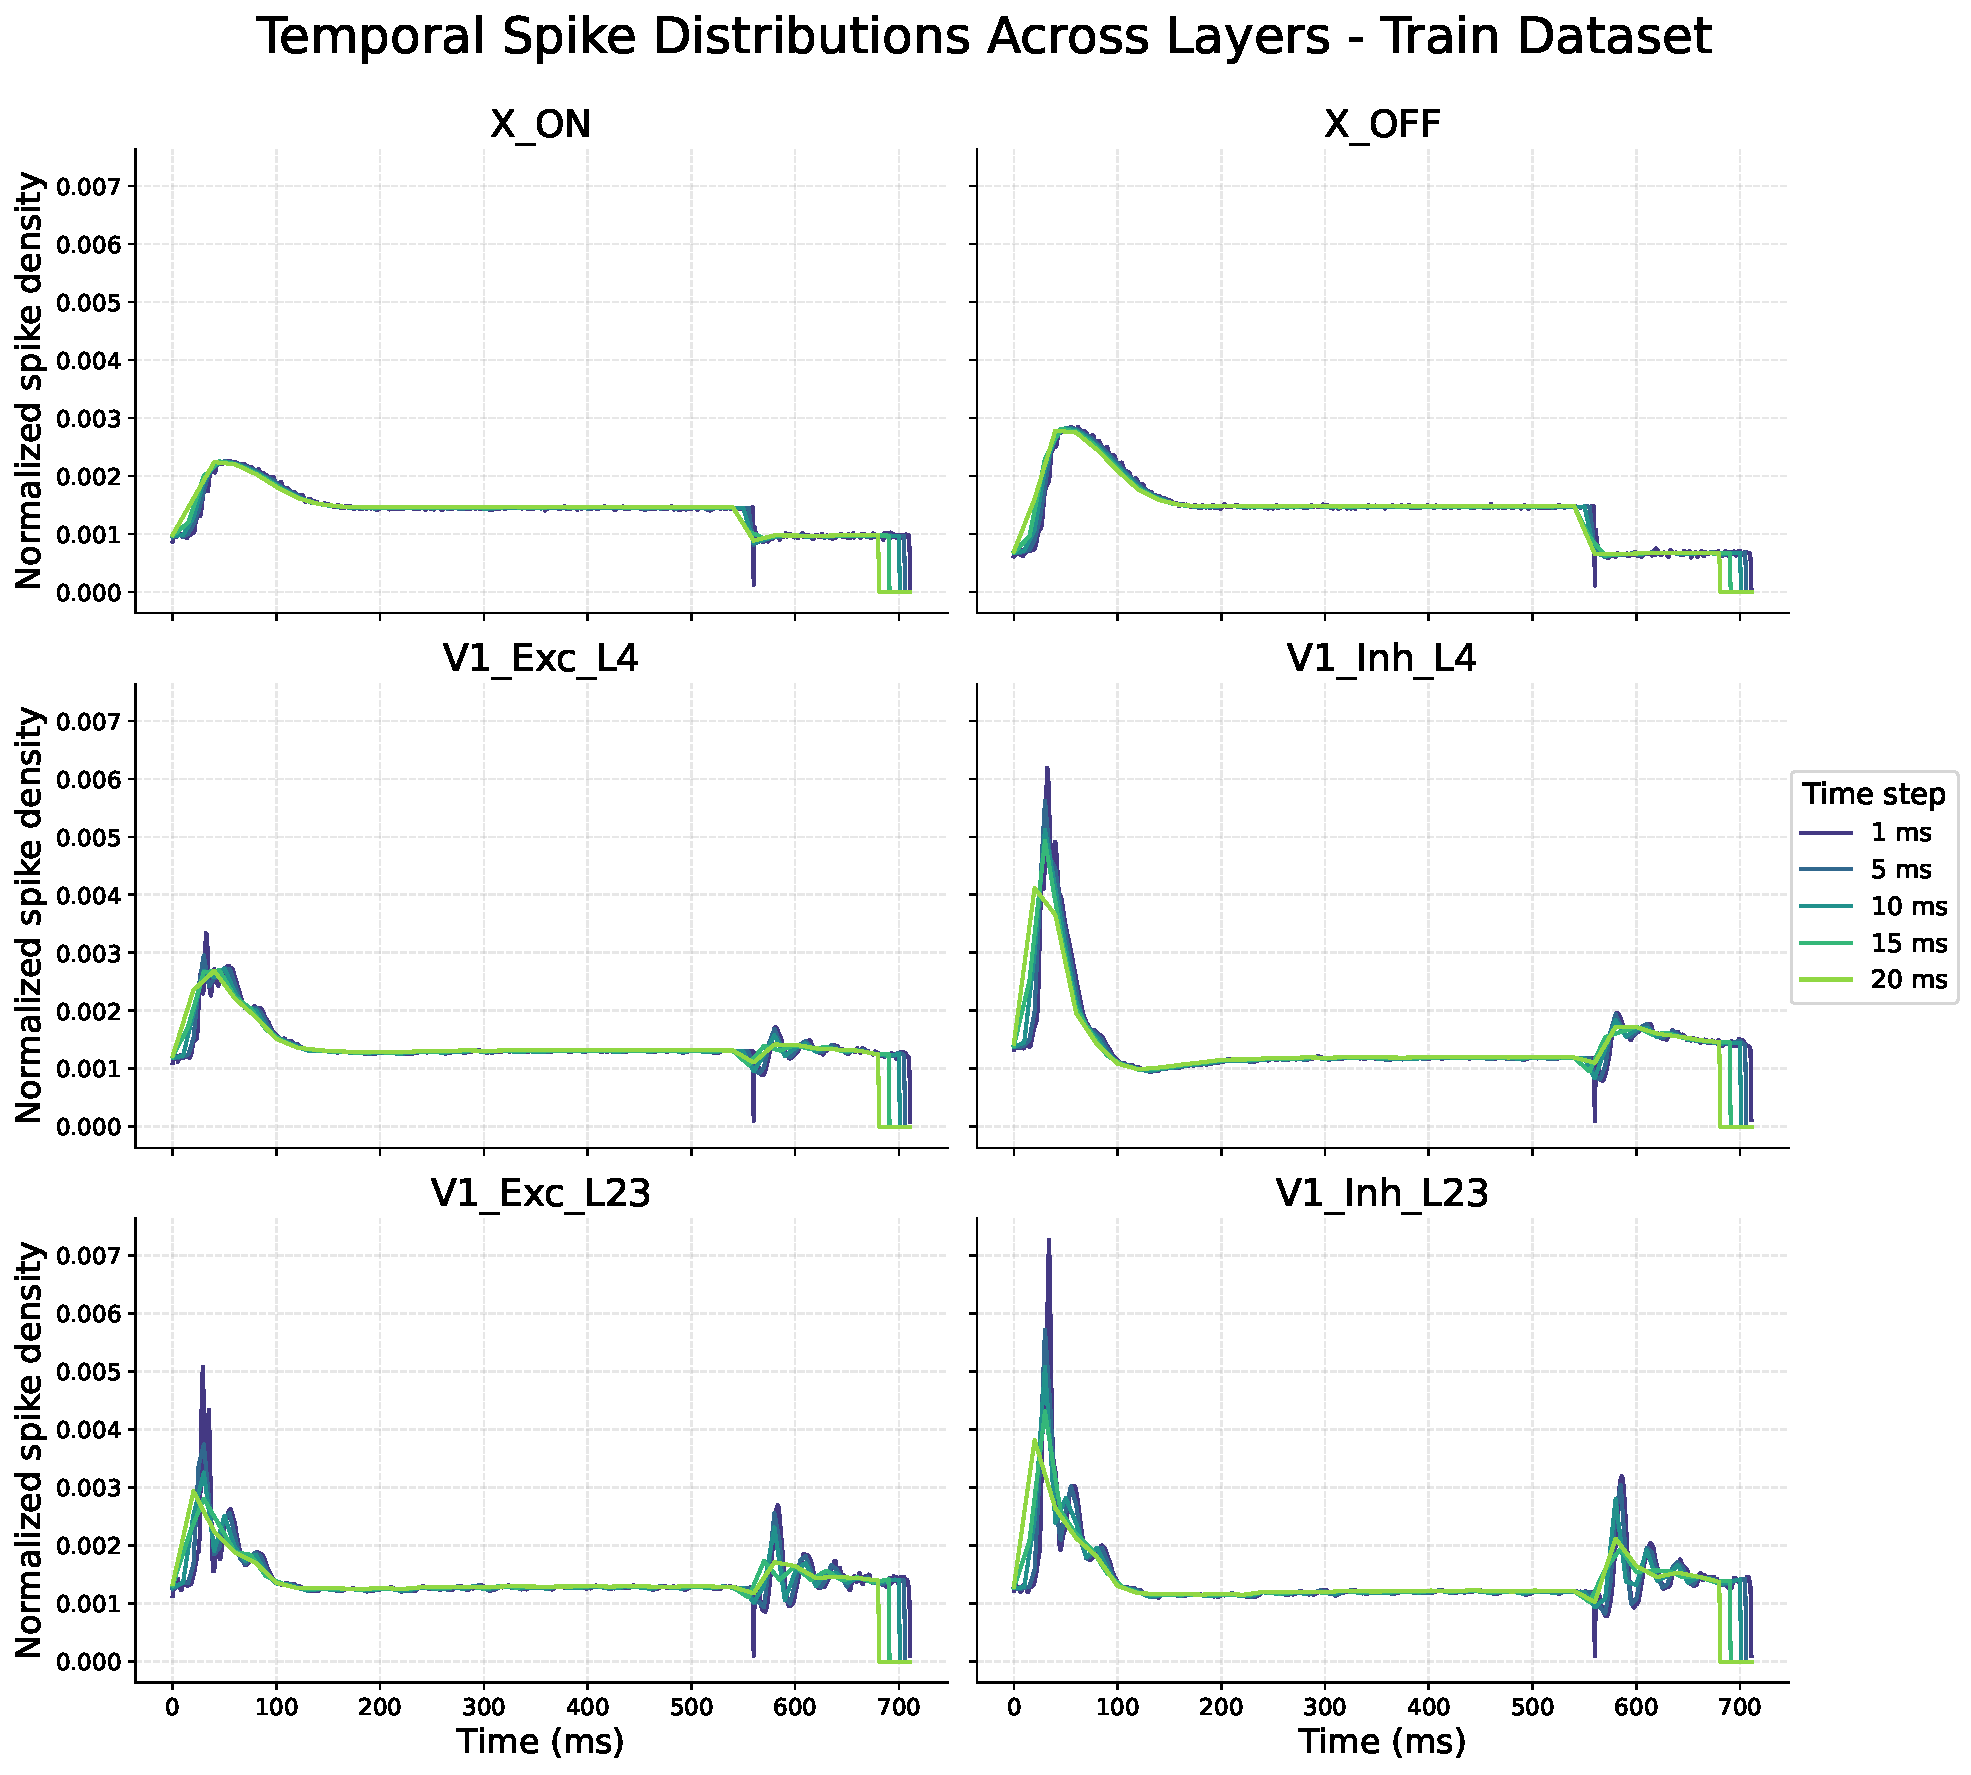
\includegraphics[width=\linewidth]{img/plots/temporal_spike_distribution_train.pdf}
    \caption{The comparison of the spike count distribution in time for different time bin sizes for all neuronal populations in train dataset. The distribution lines are interpolated to the original 1~ms distribution from the spike counts using cubic interpolation for smoothness of the line plot.}
    \label{fig:temporal_spike_distribution_train}
\end{figure}

\begin{figure}
    \centering
    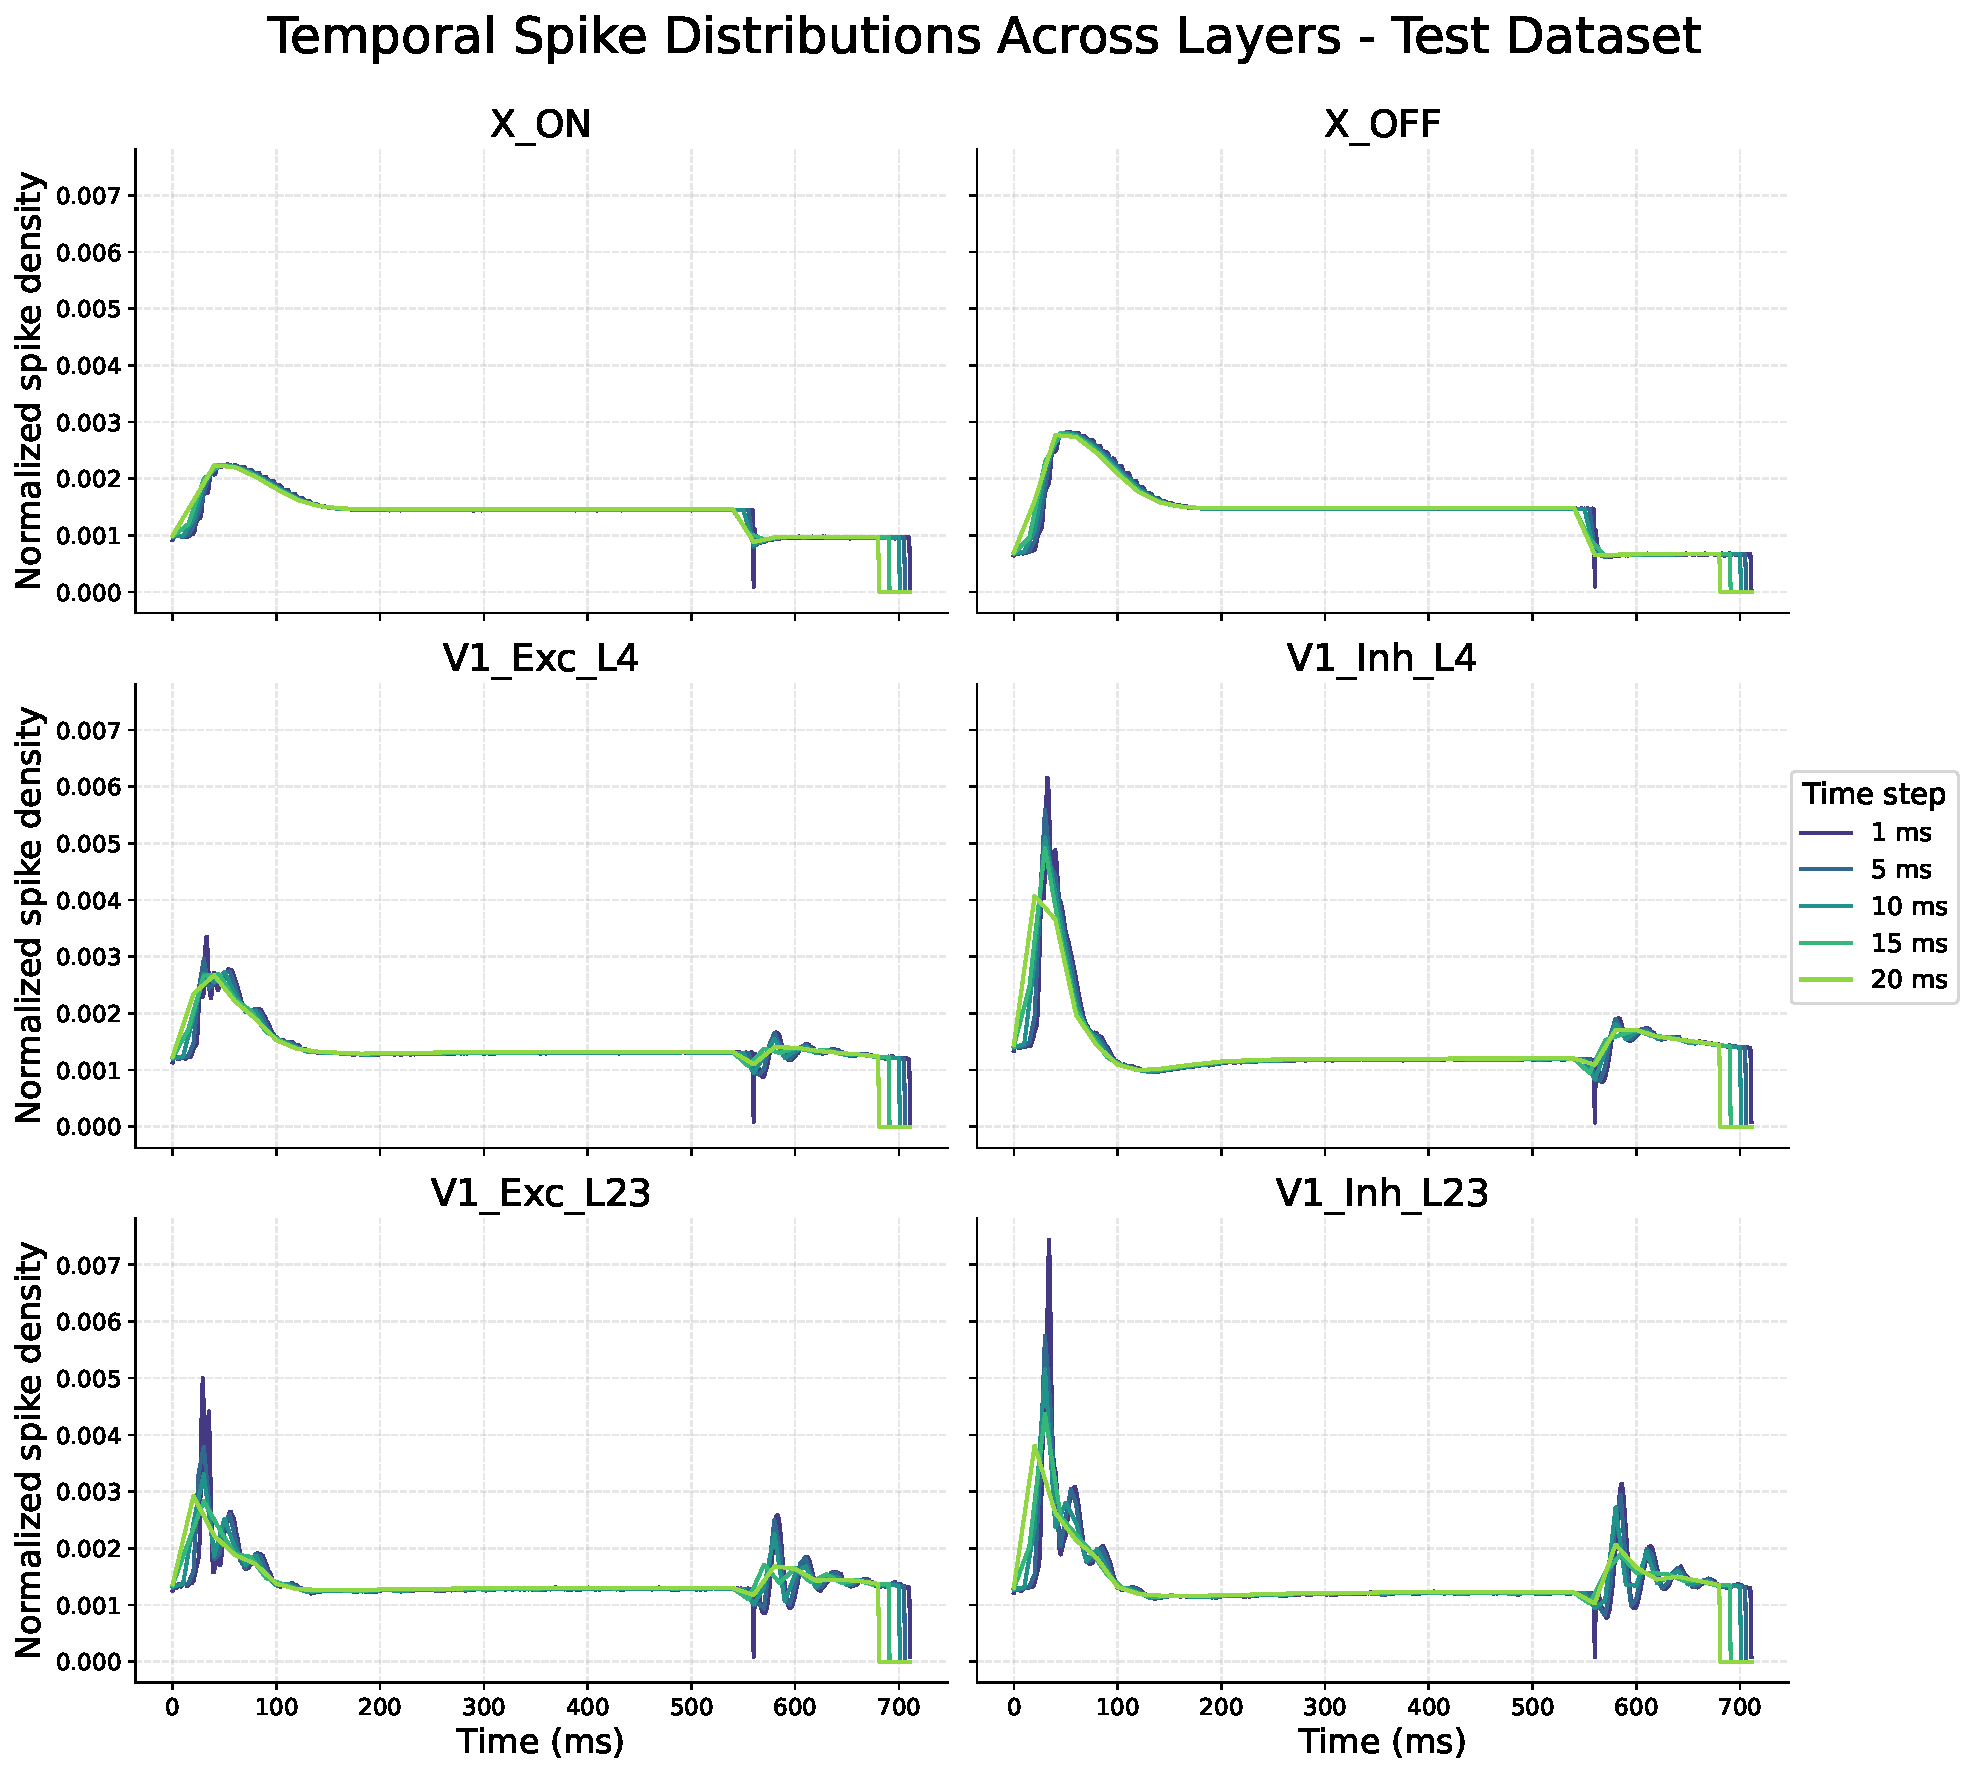
\includegraphics[width=\linewidth]{img/plots/temporal_spike_distribution_test.pdf}
    \caption{The comparison of the spike count distribution in time for different time bin sizes for all neuronal populations in test dataset. The distribution lines are interpolated to the original 1~ms distribution from the spike counts using cubic interpolation for smoothness of the line plot.}
    \label{fig:temporal_spike_distribution_test}
\end{figure}

In these plots we can clearly see that the noisiness of the count distribution clearly drops with the increasing time bin size. This phenomenon can be clearly seen especially in the excitatory layers. It is also worth noting that the training dataset seems to be noisier than the testing one. This might be caused be the much smaller ratio of data in the test dataset alongside and by the fact that in the test dataset there are multiple trials of each experiment present that might lead to smoothing of the distribution.

Furthermore, we can clearly see that the shape of the distribution remains similar across all tested time bin sizes. This is a sign that time bin merging strategy maintains the temporal properties of the data while reducing the noisiness of the data. Thus, it is sign that our merging strategy is appropriate and selection of 20~ms is a good compromise between the temporal resolution and the noisiness of the data.

To further describe the similarity of the temporal distribution of the different binning sizes, we also computed Pearson's correlation coefficients between each binning size temporal spike counts across all the neuronal layers for both train and test dataset. We visualize these using heatmaps in the Figure~\ref{fig:correlation_time_bin_size}.

\begin{figure}
    \centering
    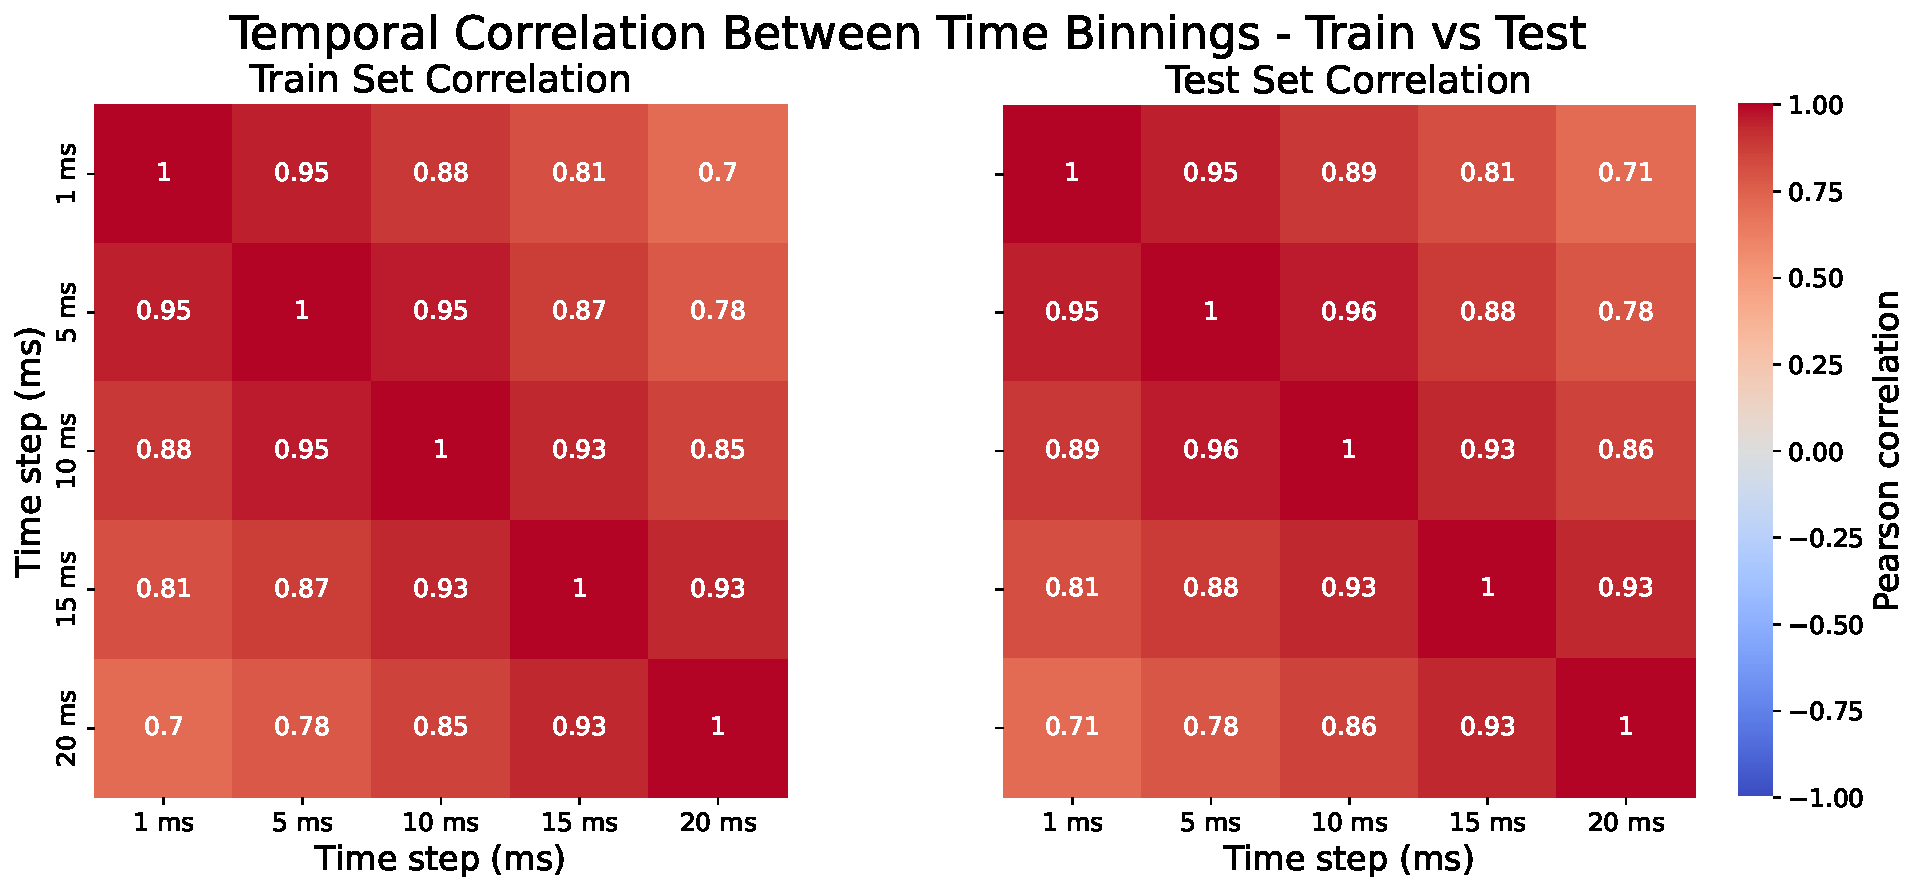
\includegraphics[width=\linewidth]{img/plots/temporal_correlation_time_bin_size.pdf}
    \caption{Heatmaps of the Pearson's correlation coefficients of the spike counts in time between different time bin sizes for train and test dataset.}
    \label{fig:correlation_time_bin_size}
\end{figure}

\subsubsection{Synchrony of Neuronal Populations in Different Time Bins}
\label{subsubsec:neuron_synchrony_binning}

Last part focused on the time binning influence is focused on the \emph{synchrony} of the neuronal populations. The synchrony is basically a measure that describes what ratio of the neuronal population fire together in the same time bin. This is an important property of the neuronal population as it can describe the temporal properties of the whole networks and is widely used in the study of the neural systems (\citet{Singer1999}). In our analysis we focus only on the mean synchrony across all time steps. We claim the following:

\begin{claim}[Synchrony of Neuronal Populations Across Time Bins]
    The mean synchrony of the neuronal populations across different time bin sizes is similar. This indicates that the temporal behavior of the neuronal responses stays roughly the same.
\end{claim}
\label{claim:synchrony_time_bins_size}

First we will plot the synchrony distributions in each layer separately for train dataset in Figure~\ref{fig:boxplot_synchrony_time_train} and for test dataset in Figure~\ref{fig:boxplot_synchrony_time_test}. The boxplots show the distribution of the mean synchrony values across all experiments. Alongside with this we also compute the mean and variance of the synchrony in time bin across all layers for different time bin sizes. The results are summarized in the Table~\ref{tab:synchrony_time_bins_summary_train} for train dataset and in the Table~\ref{tab:synchrony_time_bins_summary_test} for test dataset.


\begin{figure}
    \centering
    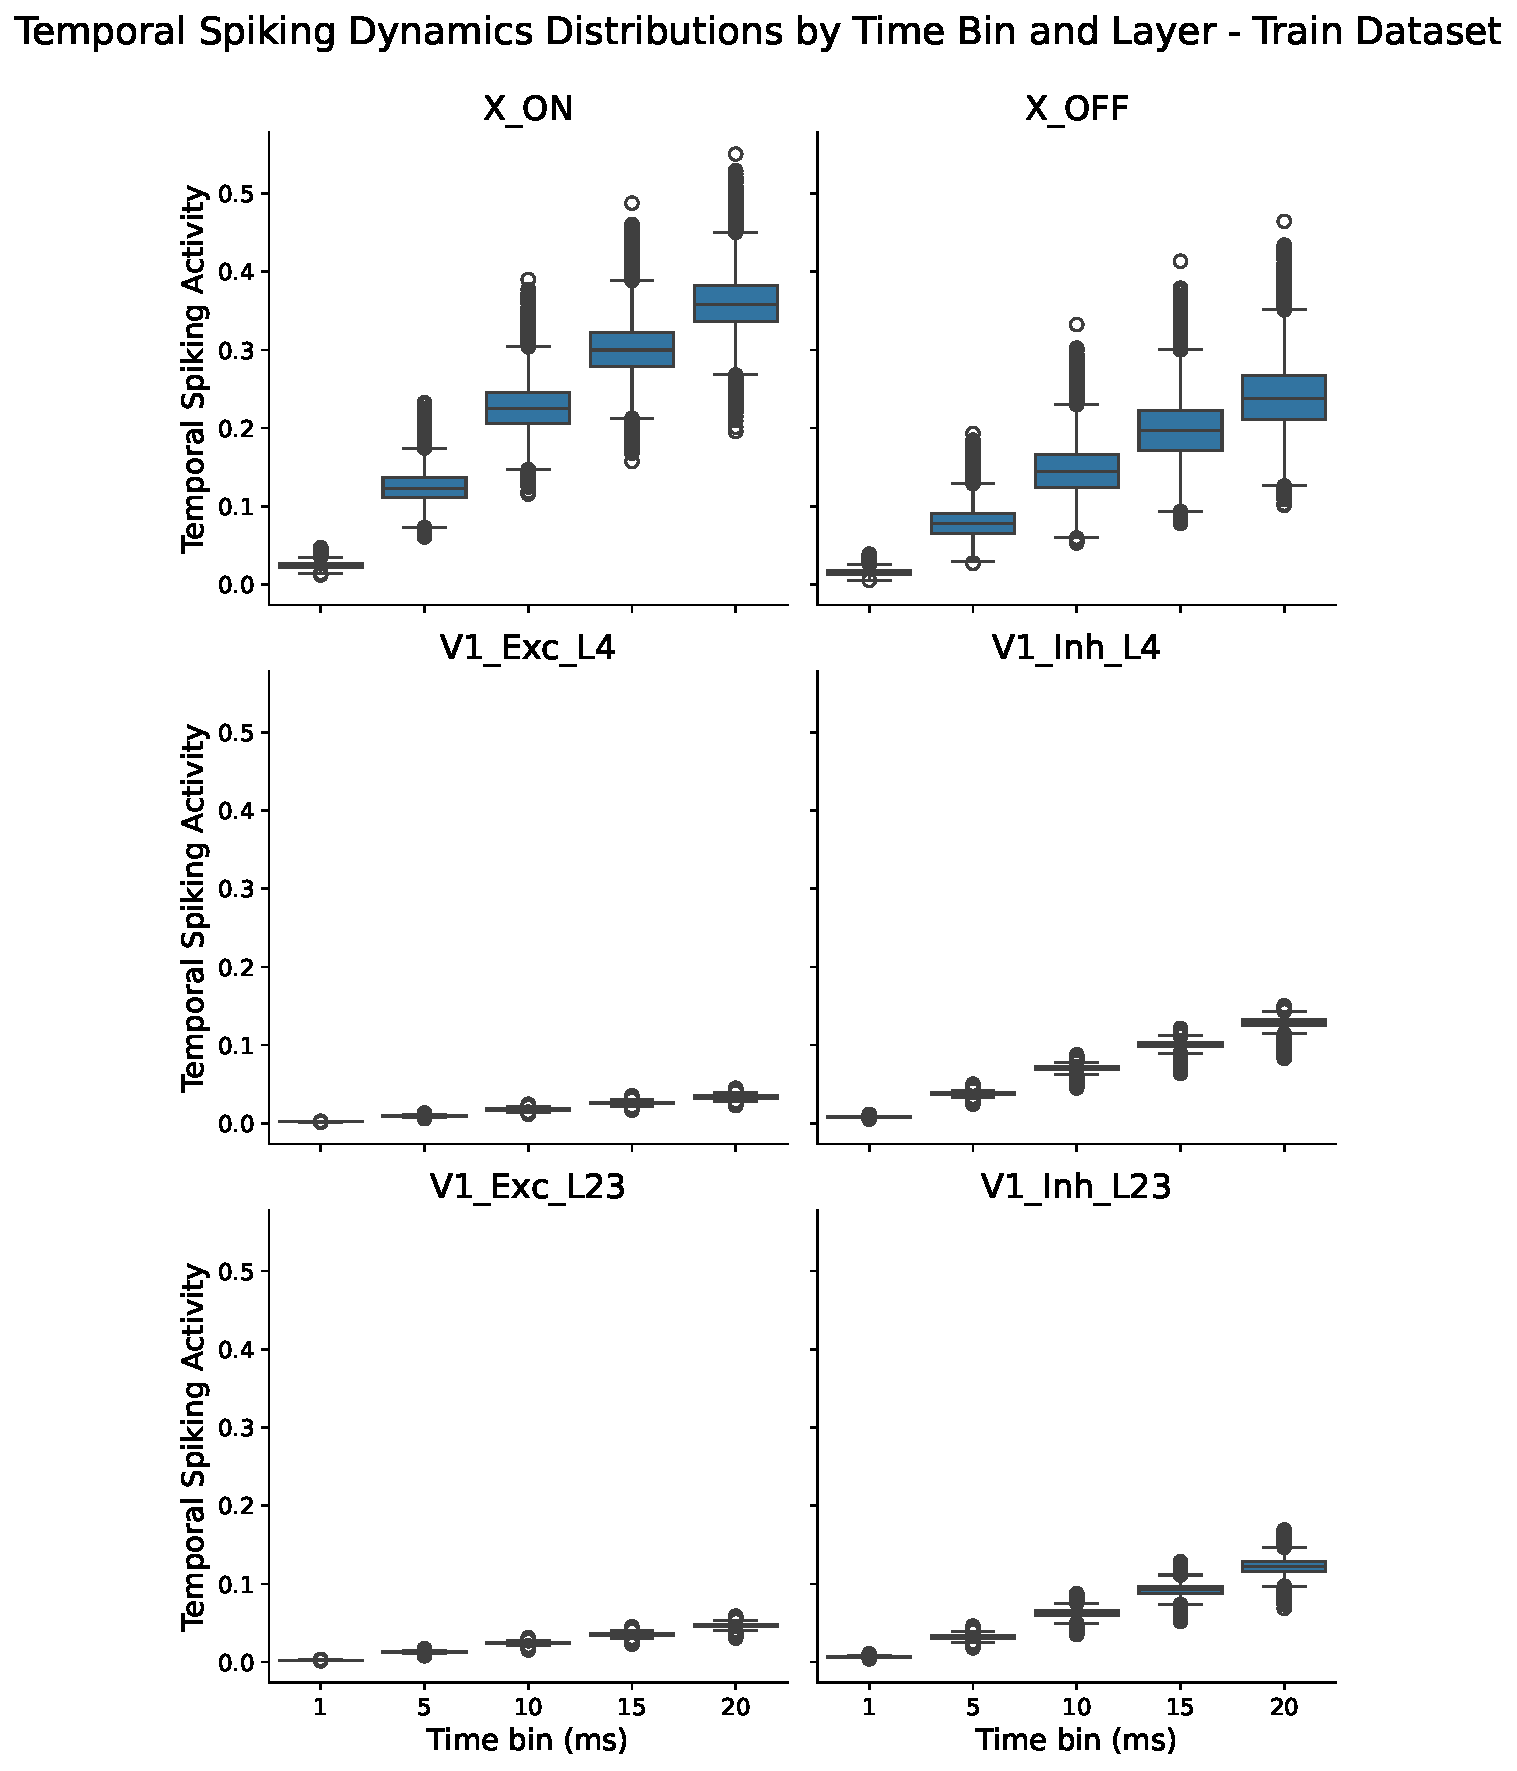
\includegraphics[width=0.92\linewidth]{img/plots/synchrony_boxplot_time_bins_train.pdf}
    \caption{Distribution of mean population synchrony of all neuronal populations across different time bin sizes for train dataset. The boxplot shows the distribution of the mean synchrony values across all experiments.}
    \label{fig:boxplot_synchrony_time_train}
\end{figure}


\begin{figure}
    \centering
    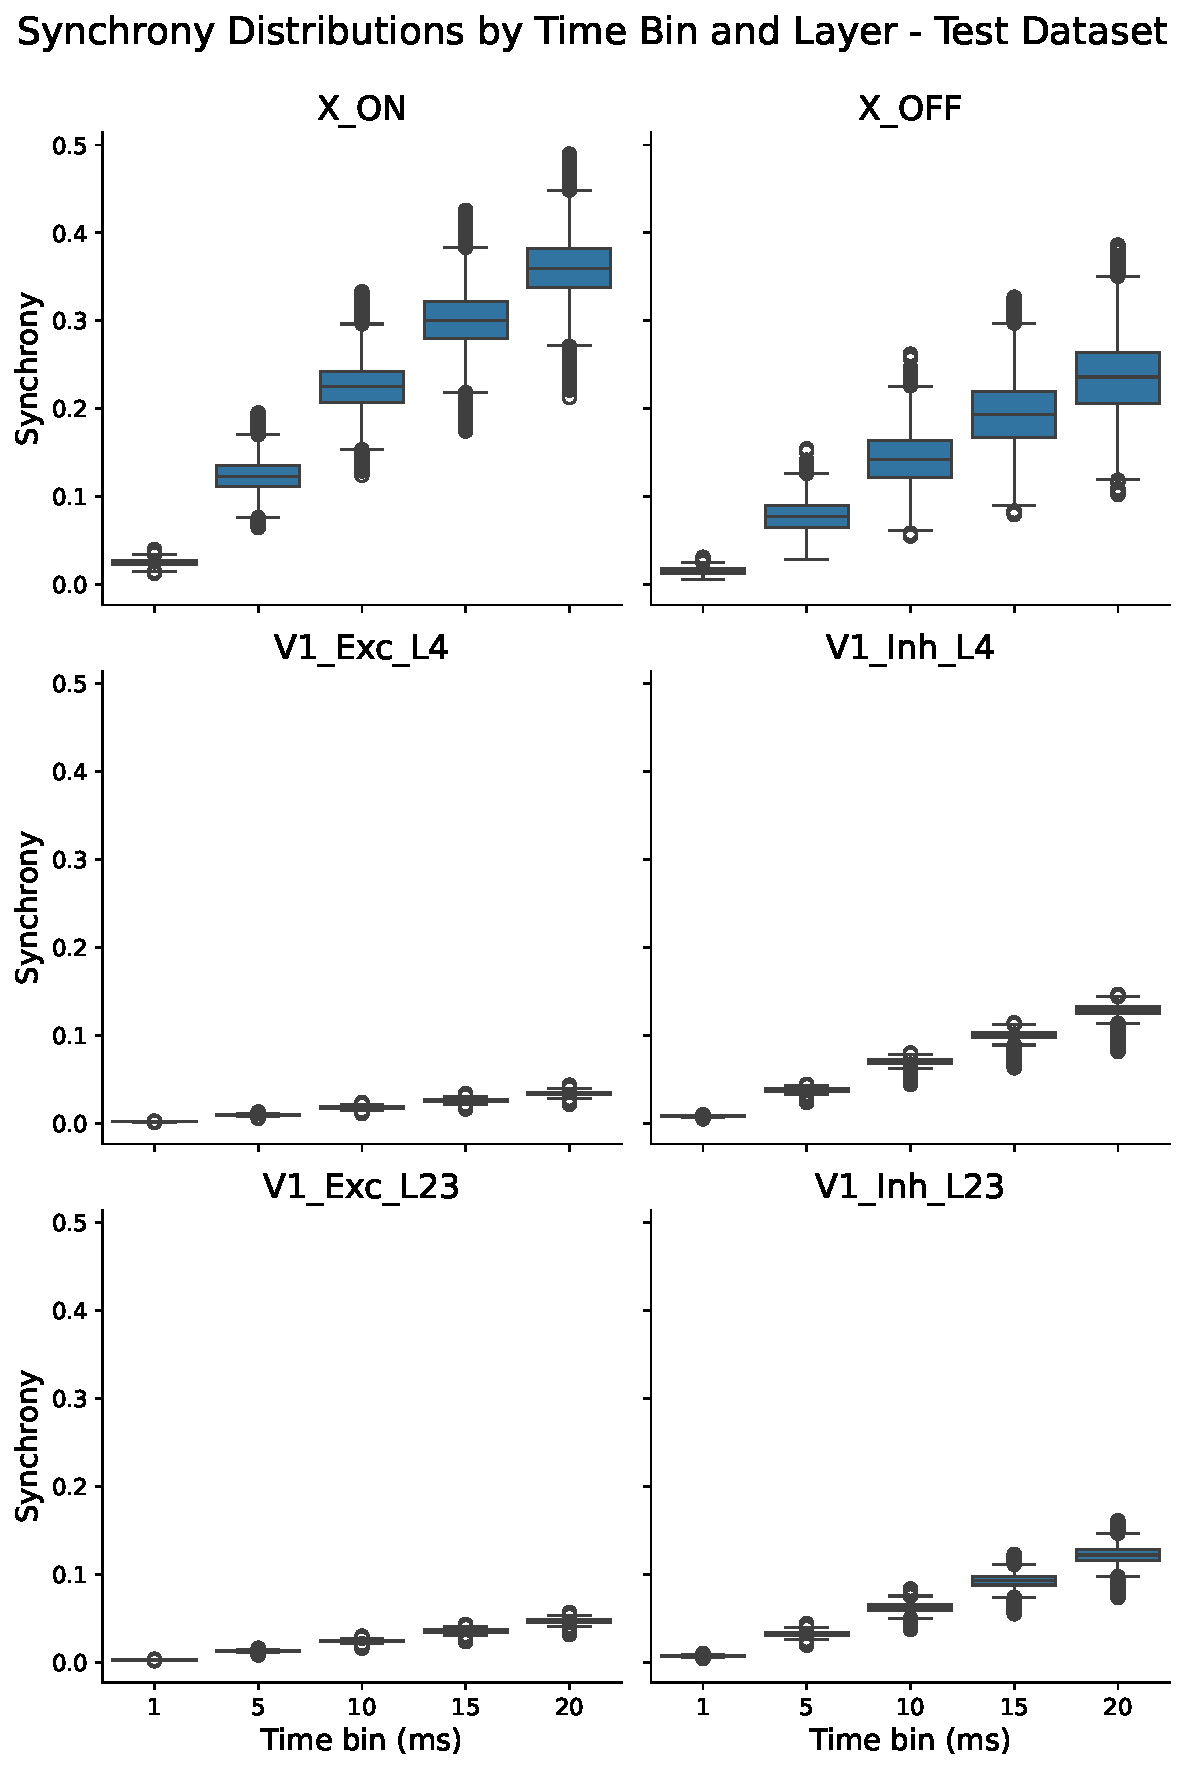
\includegraphics[width=0.92\linewidth]{img/plots/synchrony_boxplot_time_bins_test.pdf}
    \caption{Distribution of mean population synchrony of all neuronal populations across different time bin sizes for test dataset. The boxplot shows the distribution of the mean synchrony values across all experiments.}
    \label{fig:boxplot_synchrony_time_test}
\end{figure}

\begin{table}
    \centering\footnotesize\sf
    \begin{tabular}{lrr}
    \toprule
    time step & mean & variance \\
    \midrule
    1 & 0.0101 & 0.0001 \\
    5 & 0.0494 & 0.0018 \\
    10 & 0.0912 & 0.0057 \\
    15 & 0.1256 & 0.0098 \\
    20 & 0.1551 & 0.0134 \\
    \addlinespace % a nice non-intrusive separator of data groups (or final table sums)
    \bottomrule
    \end{tabular}
    \caption{\textbf{Summary of time bin synchrony statistics across all layers of train dataset:} The table depicts the mean and variance of the synchrony in time bin across all layers for different time bin sizes of the train dataset.}
    \label{tab:synchrony_time_bins_summary_train}
\end{table}

\begin{table}
    \centering\footnotesize\sf
    \begin{tabular}{lrr}
    \toprule
    time step & mean & variance \\
    \midrule
    1 & 0.0101 & 0.0001 \\
    5 & 0.0491 & 0.0017 \\
    10 & 0.0908 & 0.0057 \\
    15 & 0.1250 & 0.0097 \\
    20 & 0.1545 & 0.0133 \\
    \addlinespace % a nice non-intrusive separator of data groups (or final table sums)
    \bottomrule
    \end{tabular}
    \caption{\textbf{Summary of time bin synchrony statistics across all layers of test dataset:} The table depicts the mean and variance of the synchrony in time bin across all layers for different time bin sizes of the test dataset.}
    \label{tab:synchrony_time_bins_summary_test}
\end{table}

As we can see there is clearly a visible raise in synchrony with the larger time bin sizes. This is a sign that the larger time bins contain more spikes and thus it is more probable that more neurons will fire together more often in one time bin. As we can see there is significant raise in synchrony mainly in the LGN layers especially the layer X\_ON. On the other hand the excitatory V1 layers are effected only slightly. From these findings we can clearly see that the temporal behavior of the neuronal population is affected by the time binning and we need to be careful while interpreting the results of the model performance especially in case of the synchrony. However, despite these findings we still claim that the bin size 20~ms is the reasonable compromise between the temporal resolution, the noisiness of the data and effectiveness of the data manipulation.


\subsection{Model Subset Selection Analysis}
\label{subsec:subset_selection_analysis}
In this section we will focus on the analysis of the influence of the subset selection of the all neurons from the original SNN model. As mentioned in Section~\ref{subsubsec:subset_selection} we have selected only 10\% of the neurons from the original SNN model. This was done mainly because of the memory constraints and the computational power needed for the training of the model. We will focus mainly on the affect of the subset section on the dataset temporal properties as they are our main focus of interest in our research.

In this section we will perform the experiments exclusively on the dataset with 20~ms time bin size (as those are the ones that we use in our model) and we will focus only on the train dataset (if not stated otherwise) as we have seen  in the previous Section~\ref{subsubsec:time_bins_merging} that the test and train dataset does not really yield different results. 

\subsubsection{Total Spike Counts Across Time Bins}
\label{subsubsec:total_spike_counts_subset}
Same as in the comparison of the different time bins we will not focus on the distributions of the spike counts in time bins of the model subsets to full dataset.